\subsection{Problem in Localization}

\paragraph{}
In this project we decided to realize the challenge by a visual servoing. That is to say a line tracking by the camera. 
This type of servo control only works if the robot has at each moment the line to follow in its field of vision. 
This kind of problem can happen when the robot misses the turn. 
If the robot ever loses sight of this line, it is obvious that the challenge will not be successful. 

\paragraph{}
\paragraph{}To compensate for this unforeseen situation, we have implemented a control law that will be used as soon as the robot 
loses the line of sight sound. 
This control law requires knowledge of the robot's state.

\subsection{Robot status estimation}

\paragraph{}
To compensate for this unforeseen situation, 
we have implemented a control law that will be used as soon as the robot loses the line of sight sound. 
This control law requires knowledge of the robot's state.


\begin{figure}[!ht]
    \begin{center}
        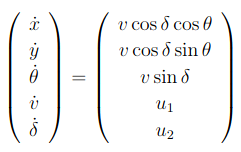
\includegraphics[scale=0.6]{Images/Etat_tricycle.png}
    \end{center}
    \caption{State of yhe robot}
    \label{fig:State}
\end{figure}

\paragraph{}
Where (x,y) is the position of the robot, $\theta$ is its heading, v its speed and $\delta$ the angle of the front wheels.
To be able to apply the Kalman filter we need a linear state representation of the robot. To make these equations linear, 
we have considered the angle $\theta$ of the robot as an input (since it is given by the inertial unit). 
This removes equation 3. Then we linearized the equation into xhat (xhat being the new state to be determined). Xhat consists of x,y, $\theta$, $\delta$. 
The file  available on our github shows the function of this Kalman filter.

